\documentclass[11pt, a4paper]{article}

\usepackage[a4paper, width = 150 mm, top = 25 mm, bottom = 25 mm]{geometry}
\usepackage{amsfonts}
\usepackage{amsmath}
\usepackage{titlesec}
\usepackage{color}
\usepackage{graphicx}
\usepackage{subcaption}
\usepackage{float}
\usepackage{verbatim}
\usepackage[style=apa,backend=biber, citestyle=authoryear, sorting=nyt]{biblatex}
\addbibresource{references.bib}

\DeclareCaptionType{equ}[][]

\title{Controlling Player Avatars and Game Worlds using Multi-Modal Input Systems}
\author{Charlie Lloyd-Buckingham}
\date{\today}


\newcommand{\addfigure}[1]
{
\hfill 

\textcolor{red}{[Add Figure: #1]}

\hfill
}

\newcommand{\commentintext}[1]
{\hfill 

\textcolor{red}{#1} 
	
\hfill
}


\newcommand{\addcitation}{\textcolor{red}{[Citation Need]}}
\newcommand{\ccite}[1]{(\citeauthor{#1}, \citeyear{#1})}
\newcommand{\cciteyear}[1]{(\citeyear{#1})}
\newcommand{\cciteauthor}[1]{(\citeauthor{#1})}
\newcommand{\reffigure}[1]{Figure \ref{#1}}
\newcommand{\reftable}[1]{Table \ref{#1}}
\newcommand{\refequation}[1]{Equation \ref{#1}}


\begin{document}

% Controlling Player Avatars in Game Worlds using Multi-Modal Input Systems
\maketitle



\pagebreak
\section{Acknowledgements}	

A thank you to my supervisors, Fred Charles and Simant Prakoonwit for guiding me in the completion of this dissertation. Alongside my girlfriend Rianna Green and friends Paul Brown, Sam Neville, Areej Ammar and Chevontia Raju for both moral and technical support through out my final year.

\section{Abstract}	

Input methodologies for video games have adapted over the years as different technologies have become more accessible around the world. With the growing usage of video games within academic research and the pairing of these games with EEG and EMG technologies, this dissertation asks the question, why haven't major console manufactures developed systems with these technologies yet. 

\hfill

By combining these technologies into a single system for in game interactions via the usage of the Lab Streaming Layer (LSL) and Feed Forward Neural Networks (FFNNs), two example use cases where designed. The first was for motor imagery based avatar control and the second a simple adaptive difficultly system. These were used to demonstrate the potential of using these technologies within a the gaming industry as consumer products. The results suggested that a greater look into a more complex solution may be required when classifying motor imagery data and a players performance, due to the inaccuracy of the FFNNs used within the project.



\pagebreak
\tableofcontents				% - 300 Words



% Introducition and Context, Including Aim's and Objectives
\pagebreak
\section{Introduction}	
\subsection{Context}

Throughout the history of the games industry, game makers have been exploring new ways to deliver their players unique experiences. This has come in the forms of the narrative decisions within a game's story, stylistic decisions through the game's art and, as a focus for this dissertation, the interaction systems designed around the player's influence within a game's world. 

\hfill

On account of the digital nature of video games, as technology has evolved over the years, so too has the hardware and methods of interaction used within gaming consoles. Beginning in 1972 with the creation of the first home console, the Magnavox Odyssey, over the following years, video game console manufactures have continued to push the perceived boundaries of interactive entertainment. In 2006, Nintendo demonstrated the potential of a motion controlled input system with the Wii. Following this, other manufactures also began to expand into the technology, with Microsoft developing the Xbox Kinect and Sony the PlayStation Move. Nowadays, companies like Oculus and the HTC corporation are exploring the market of consumer virtual reality (VR) headsets with the Quest and Vive, while Nintendo is continuing to adapt new ways of using motion technology within their Labo Toycon games. All of this has demonstrated that with the market's continued interest in new experiences, console manufactures and game developers will continue innovating new methods of interaction for their players.

\subsection{Research Problem}

There has also been a growing interest in the usage of electroencephalographic (EEG) and electromyographic (EMG) techniques being coupled with game engines for the purpose of research. The use of games in research has been invaluable for decades, due to the added flexibility and control given when stimulating a subject. The act of reversing this dynamic and using one of these devices, as shown with EEG by Marshall and colleagues \cciteyear{6518141}, for the purpose of entertainment has been explored, however there is still yet be any consumer ready solution to come from this. 

\subsection{Project Aims}

It is with this in mind, that this dissertation proposes to continue with the investigation into the viability of using EEG, EMG, and VR as input modalities within a video game. By acquiring data from multiple devices and combining them, the aim is for the creation of a single system capable of attaining and extracting meaningful interactions from it's users for control over aspects of game world. Alongside this, two example games will also be constructed, these will be used to verify if the system is capable of performing it's tasks correctly and potentially demonstrate a working example from within a use-case environment.

\pagebreak
\subsection{Project Objectives}

To get this system working, data from each device will need to be accessed live and streamed into the Unity game engine where a pre-trained feed forward neural network (FFNN) will be used to decipher a meaning suitable for the given game. From this the two games will be developed: the first will have the player use motor imagery to control the limbs of a virtual avatar; the second game will use the system measure the users state of mind, allowing for adaptive difficulty depending on the focus of the player. These two solutions would allow for testing the viability of using a system like this as either a direct method for controlling a game, as well as the usefulness in altering a games state to increase player enjoyment and engagement.

% Review of Literature and / or Proffesional Practices
\pagebreak
\section{Research}	
\subsection{Literature Review}	% - 2000 Words

The usage of multi-modal input systems is not unheard of, almost all modern first person console shooters use the input controller's built in gyroscope, in addition to the right joystick to control the direction of the players camera. This multi-input system allows much more finesse when aiming, resulting in the players having a more enjoyable experience \ccite{toktacs2019evaluation}. In the work put forward by Silva and Amaral \cciteyear{da2014multimodal}, they demonstrate that the inclusion of a multi-modal input system compared to a uni-modal input system can make video games perceivably more enjoyable, ``It can be used to increase the feeling of empowerment on the player when using certain abilities, or to intentionally make in-game actions more difficult by demanding more physical effort from the player''. Though gyroscopic-assisted aiming is a more recent phenomenon, the concept of incorporating multiple input systems for singular interactions within gaming has been around for a while. Even back in 2009 with the release of `The Legend of Zelda: Spirit Tracks' \ccite{thelegendofzelda_spirittracks}, when using the flute, players would be required to both blow into the DS microphone and use the touch screen to play specific tones. This interaction could have very easily be performed by mapping tones to regions on the touch screen, or pairing each tone to a button on the Nintendo DS, much like how previous instruments in the franchise have been implemented, E.g. `The Legend of Zelda: Majoras Mask' \ccite{thelegendofzelda_majorasmask}. However, as stated by Silva \cciteyear{da2014multimodal}, players could have a ``feeling of empowerment'' overcoming the set-pieces Nintendo designed, through this added multi-modal challenge.

\hfill

Before looking into EEG as a part of a larger multi-modal input system, a focus on how it has been used on its own within video gaming will be explored. Games using EEG most commonly occur in the form of serious games, defined by Alvarez and colleagues \cciteyear{alvarez2011introduction} as a video game that is ``intended to depart from the simple entertainment''. This refers to games built for research, education and rehabilitation. Whether this is just for providing an environment for the comparison between different electroencephalographs \ccite{liarokapis2014comparing}, evaluating a participant's emotions and satisfaction \ccite{vourvopoulos2013brain}, screening for early signs of mental illness \ccite{tarnanas2015comparison}, or cognitive rehabilitation \ccite{alchalcabi2017more}. 

The data captured from EEG can be used in a multitude of ways, depending on what is considered important for a given experiment. By using games it is then possible to focus on these targeted aspects of EEG: allowing for the invocation of responses necessary for measuring event related potentials \ccite{ahn2011using}, or to provide a real-time environment capable of demonstrating the changes in mental states \ccite{liarokapis2015examining} and motor-imagery \ccite{ndulue2019driving}. 

However, it is debated whether EEG technology is still in it's infancy \ccite{rashid2020current}. When investigating the current state of brain computer interfaces (BCIs) usability in the context of information transfer rates (ITR), Rashid and colleagues \cciteyear{rashid2020current} write ``In spite of the many outstanding breakthroughs that have been achieved in BCI research, some issues still need to be resolved... the existing BCIs offer somewhat poor ITR for any type of effectual BCI application'', while in Cattan's \cciteyear{cattan2021use} comparison, they state ``In practice, this means that BCIs are unusable in traditional inputs, such as in keyboards or mice''. To the contrary, EEG technology has already been used within for video games as an interactive medium: from modifying a game's difficulty based on the focus of the player with Tetris \ccite{liarokapis2015examining}; walking around the streets of Ancient Rome using motor-imagery in Rome Reborn \ccite{ndulue2019driving}; to piloting a space ship in Rock Evaders \ccite{ndulue2019driving}. This is evidence of the potential that EEG has as a method of input for video games.

\hfill

The usage of EMG within video games has also been quite extensive. EMG based serious games have permitted the research of various topics, from measuring arousal to stimuli using the muscles in the face \ccite{schuurink2008engagement}, to the effectiveness of myoelectric prosthesis training \ccite{bessa2020designing}. While their use outside of research has aided in the rehabilitation of patients, suffering: post injury \ccite{gutierrez2020serious} \ccite{schonauer2011full}; strokes \ccite{ghassemi2019development} and other medical disorders \ccite{labruyere2013requirements}. Though much more infrequent, entertainment focused EMG games do exist. In large part with they goal for allowing people with motor impairments to have the opportunities to play games, Kamau-Mugro \cciteyear{muguro2020development} states ``Focusing on neck EMG, would give more control to individuals with hand disabilities or SCI [Spinal Cord Injury] patient as a control scheme or an entertainment interface''.

\hfill
  
Having investigated the viability of EEG and EMG as uni-modal input systems, this dissertation will explore their combined usage alongside other additional input modalities. Though the appearance of entertainment based multi-modal EEG and EMG systems are infrequent, multi-modal serious games using EEG and EMG are a lot more common. An example of which is Sivanathans \cciteyear{sivanathan2014temporal} work on multi-modal EEG analysis, in which data from in-game events was coupled with the EEG input streams to allow for a greater understanding of the results. Though there aren't many instances of multi-modal EEG and EMG based video game systems, that isn't to say inspiration for these systems cannot come from elsewhere, the majority of research in which multi-modal EEG and EMG systems have been built for is in the development of consumer prosthetics \ccite{shi2019novel} and wheelchair controllers \ccite{carlson2013brain}. These systems pull from the data streams of EEG and EMG and by using eye-tracking, computer vision and inverse kinematics \ccite{mcmullen2013demonstration} are able to allow for finer control over hardware systems that on their own EEG and EMG wouldn't be able. By adopting a similar approach, these real world solutions can be used with virtual controllers instead. 

\hfill

Understanding meaning from EEG and EMG data is complex. To get around this, several studies have opted for the use of machine learning. An example of the technology used for classification of this data, is the FFNN. Jana and colleagues \cciteyear{jana2018enhancing} demonstrate the usefulness of FFNNs by showing a higher accuracy when compared against other networks, using motor imagery classification. The same can be said for the usefulness of the FFNN within the classification of a participant's state of mind as shown by Makeig and colleagues \cciteyear{makeig1995using}, highlighting alertness. 

\hfill

With the combination of these technologies and the processing of the data, interference on an individual level becomes a main concern can be. Blinking is a cause for a large amount of EEG interference \ccite{kasim2022effective} "Ocular artifact is the most common and critical EEG artifact. These artifacts generate enormous potentials and can occur about 20 times per minute and continue between 50 and 500 ms", during the runtime of an application, this misfiring of sensors can cause a lot of unwanted affects. With a combined system however, the detection of sources of interference can performed and its effects nullified. Using EMG, the tracking of ocular movement may be performed via the sampling of the orbicularis obuli muscle \ccite{frigerio2014surface}. These movements can then be fed into a neural network and with the right training, blinks can be detected \ccite{erkaymaz2015detection} and used to remove the affected samples of EEG. 





\pagebreak
\section{Methodology and Process}			% - 5100 Words

In this section, the design and implementation of both the system and example game will be discussed. The system, shown in \reffigure{fig:system_diagram_:_generic}, will be devised to allow for the retrieval of real-time data from three input devices: the Emteq Pro, for sampling the EMG data; the eego sports, for sampling EEG data; and a compatible VR headset, for tracking player position and orientation. Following this, the input data would then be passed directly to the application or distributed across the local network where through the use of machine learning, a meaning would be construed and used in a way to affect the game.



\begin{figure}[H]
	\centering
	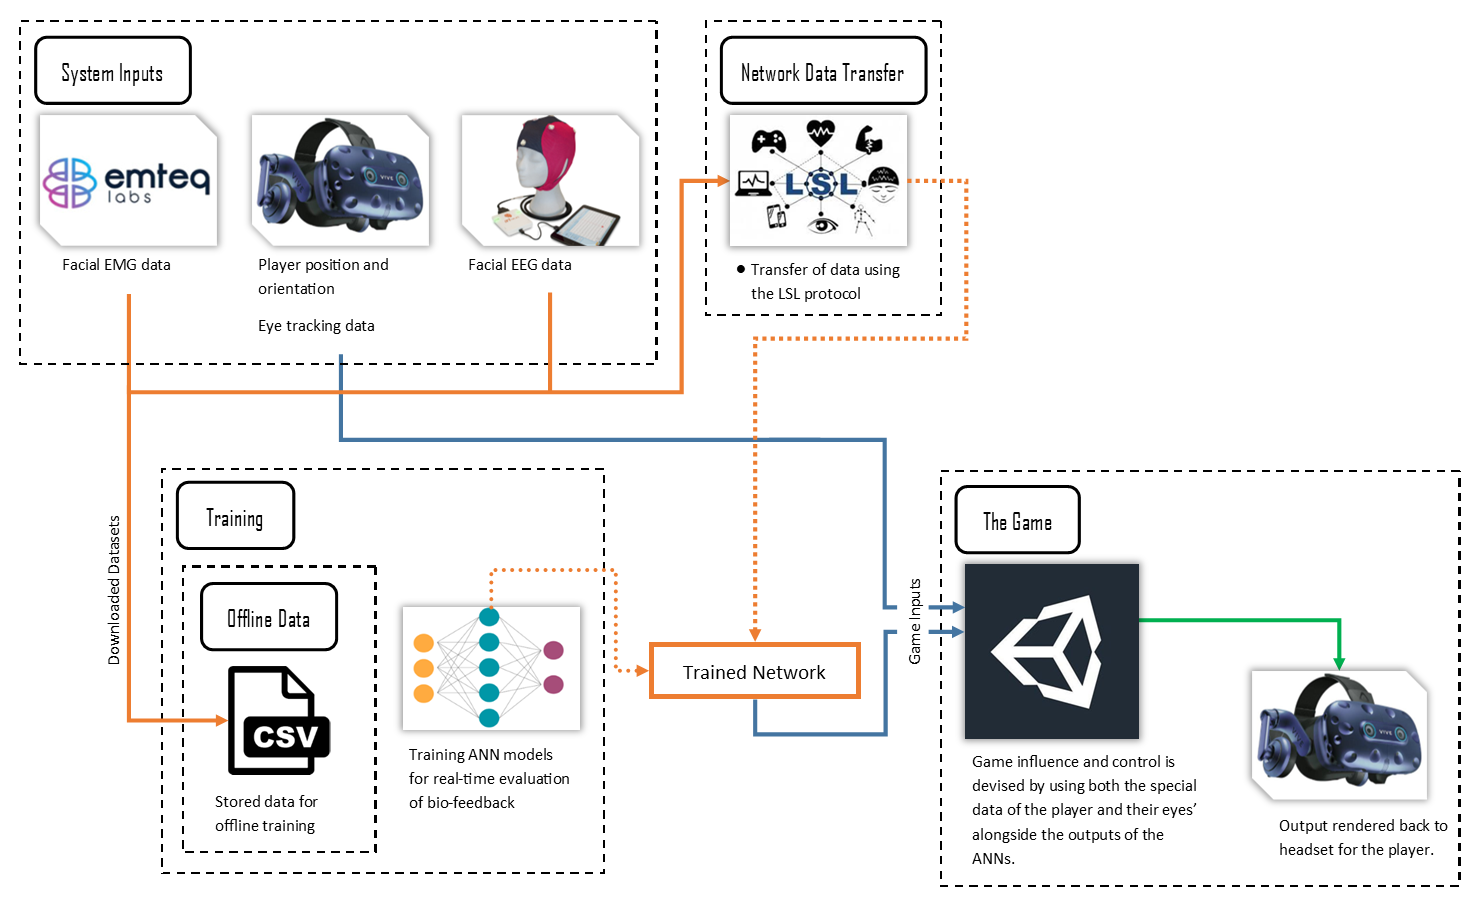
\includegraphics[width = 0.9 \linewidth] {[ Figures ]/System Diagram.png}
	\captionsetup{font = small, labelfont = small, width=.8\linewidth}
	\caption{System diagram: How input data from the specified technologies will be accessed and used within the game.}
	\label{fig:system_diagram_:_generic}
\end{figure}



The game was developed in the game engine Unity 3D. To use the data from the VR, EEG and EMG devices, each technology was integrated into the engine using C\#, and a variety of packages provided by and for Unity. The game itself consisted of a pair of two mini-games, both focusing on potential aspects of how a system like this could reasonably be used in a real world example. 


\begin{figure}[H]
	\centering
	\begin{subfigure}[t]{0.45\linewidth}
		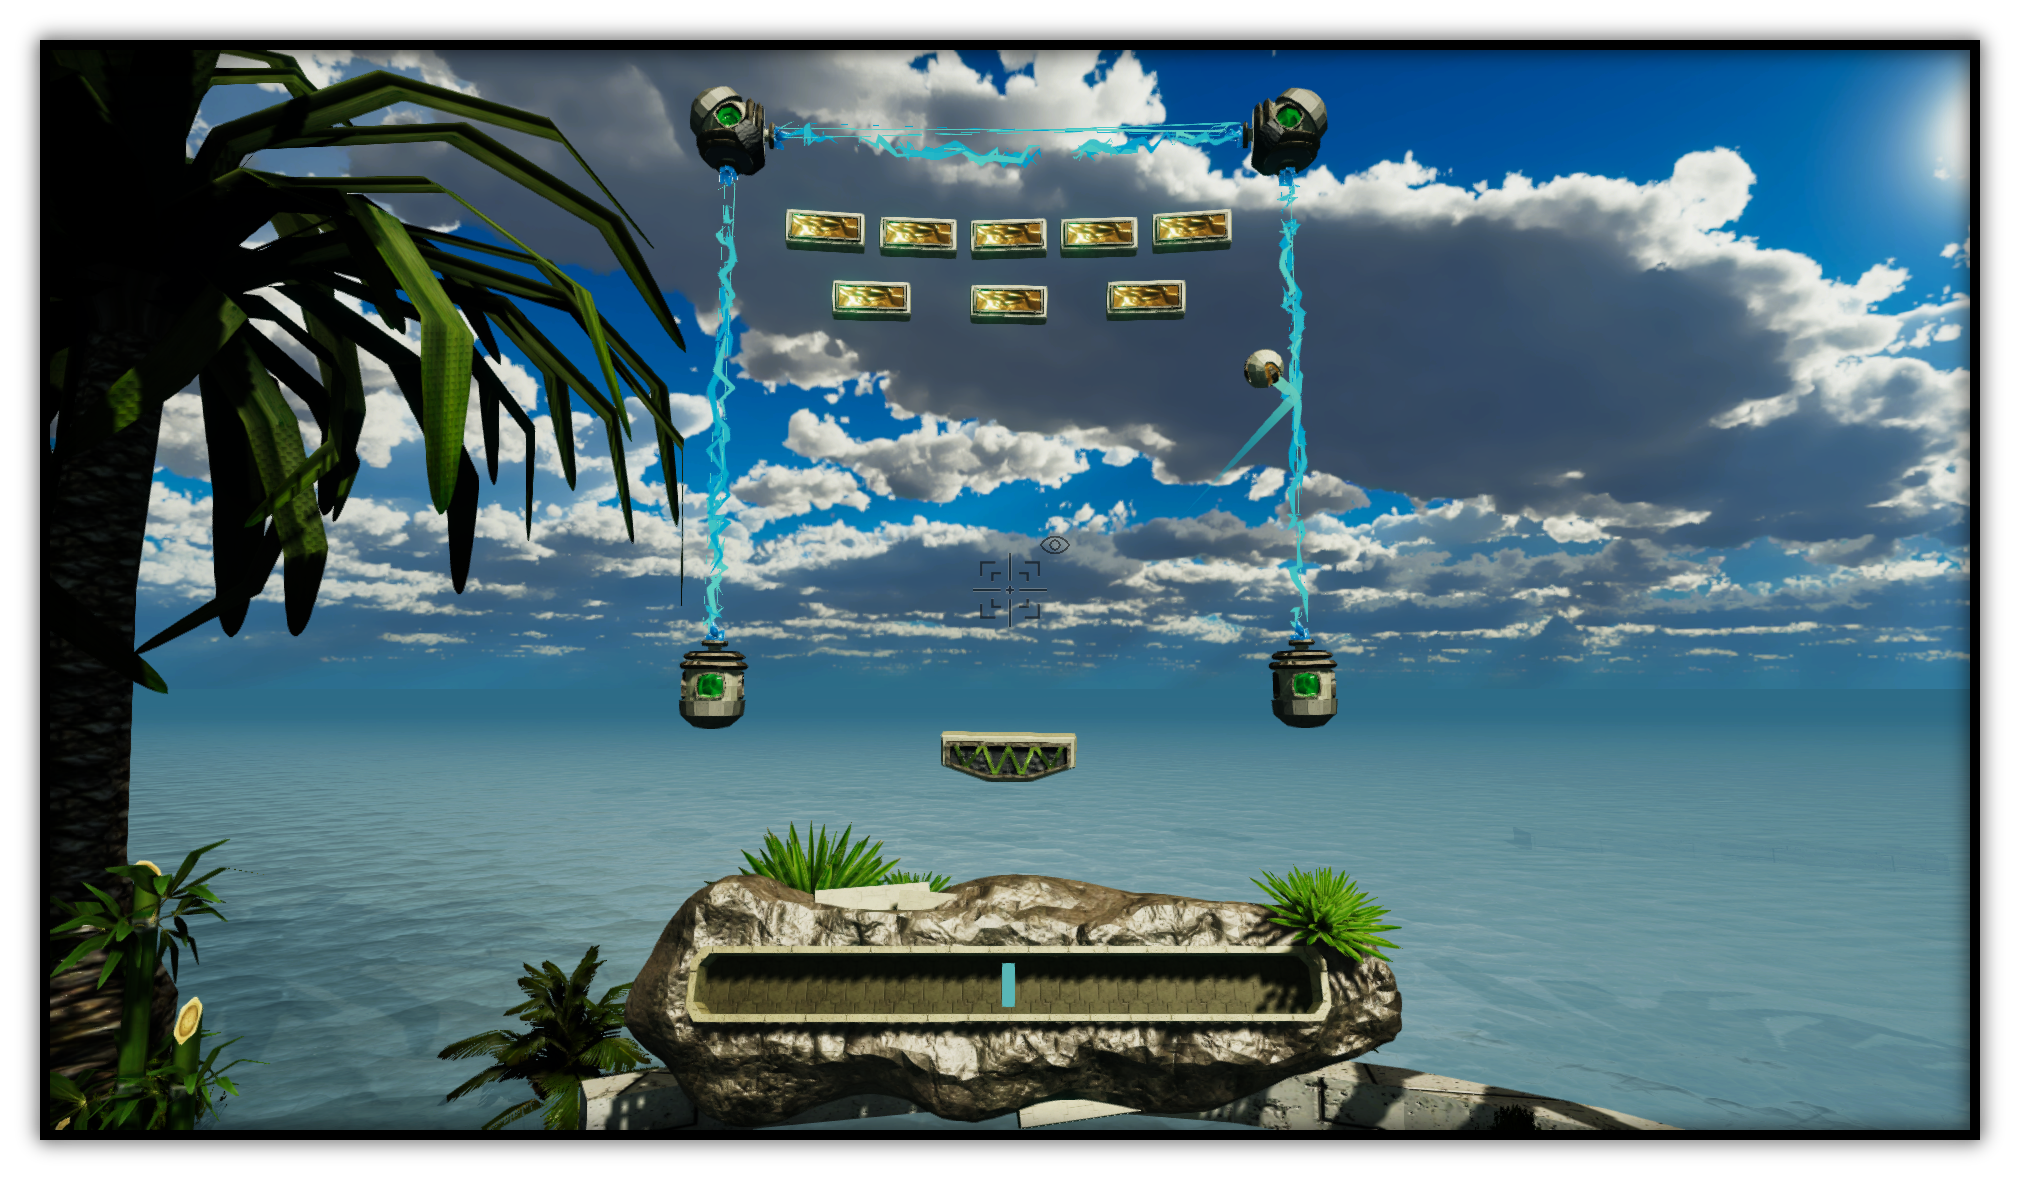
\includegraphics[width = \linewidth] {[ Figures ]/Breakout Mini-Game.png}
		\captionsetup{font = small, labelfont = small, width=.8\linewidth}
		\caption{Breakout: concentration based adaptive difficulty.}
		\label{fig:the_game_1}
	\end{subfigure}
	\begin{subfigure}[t]{0.45\linewidth}
		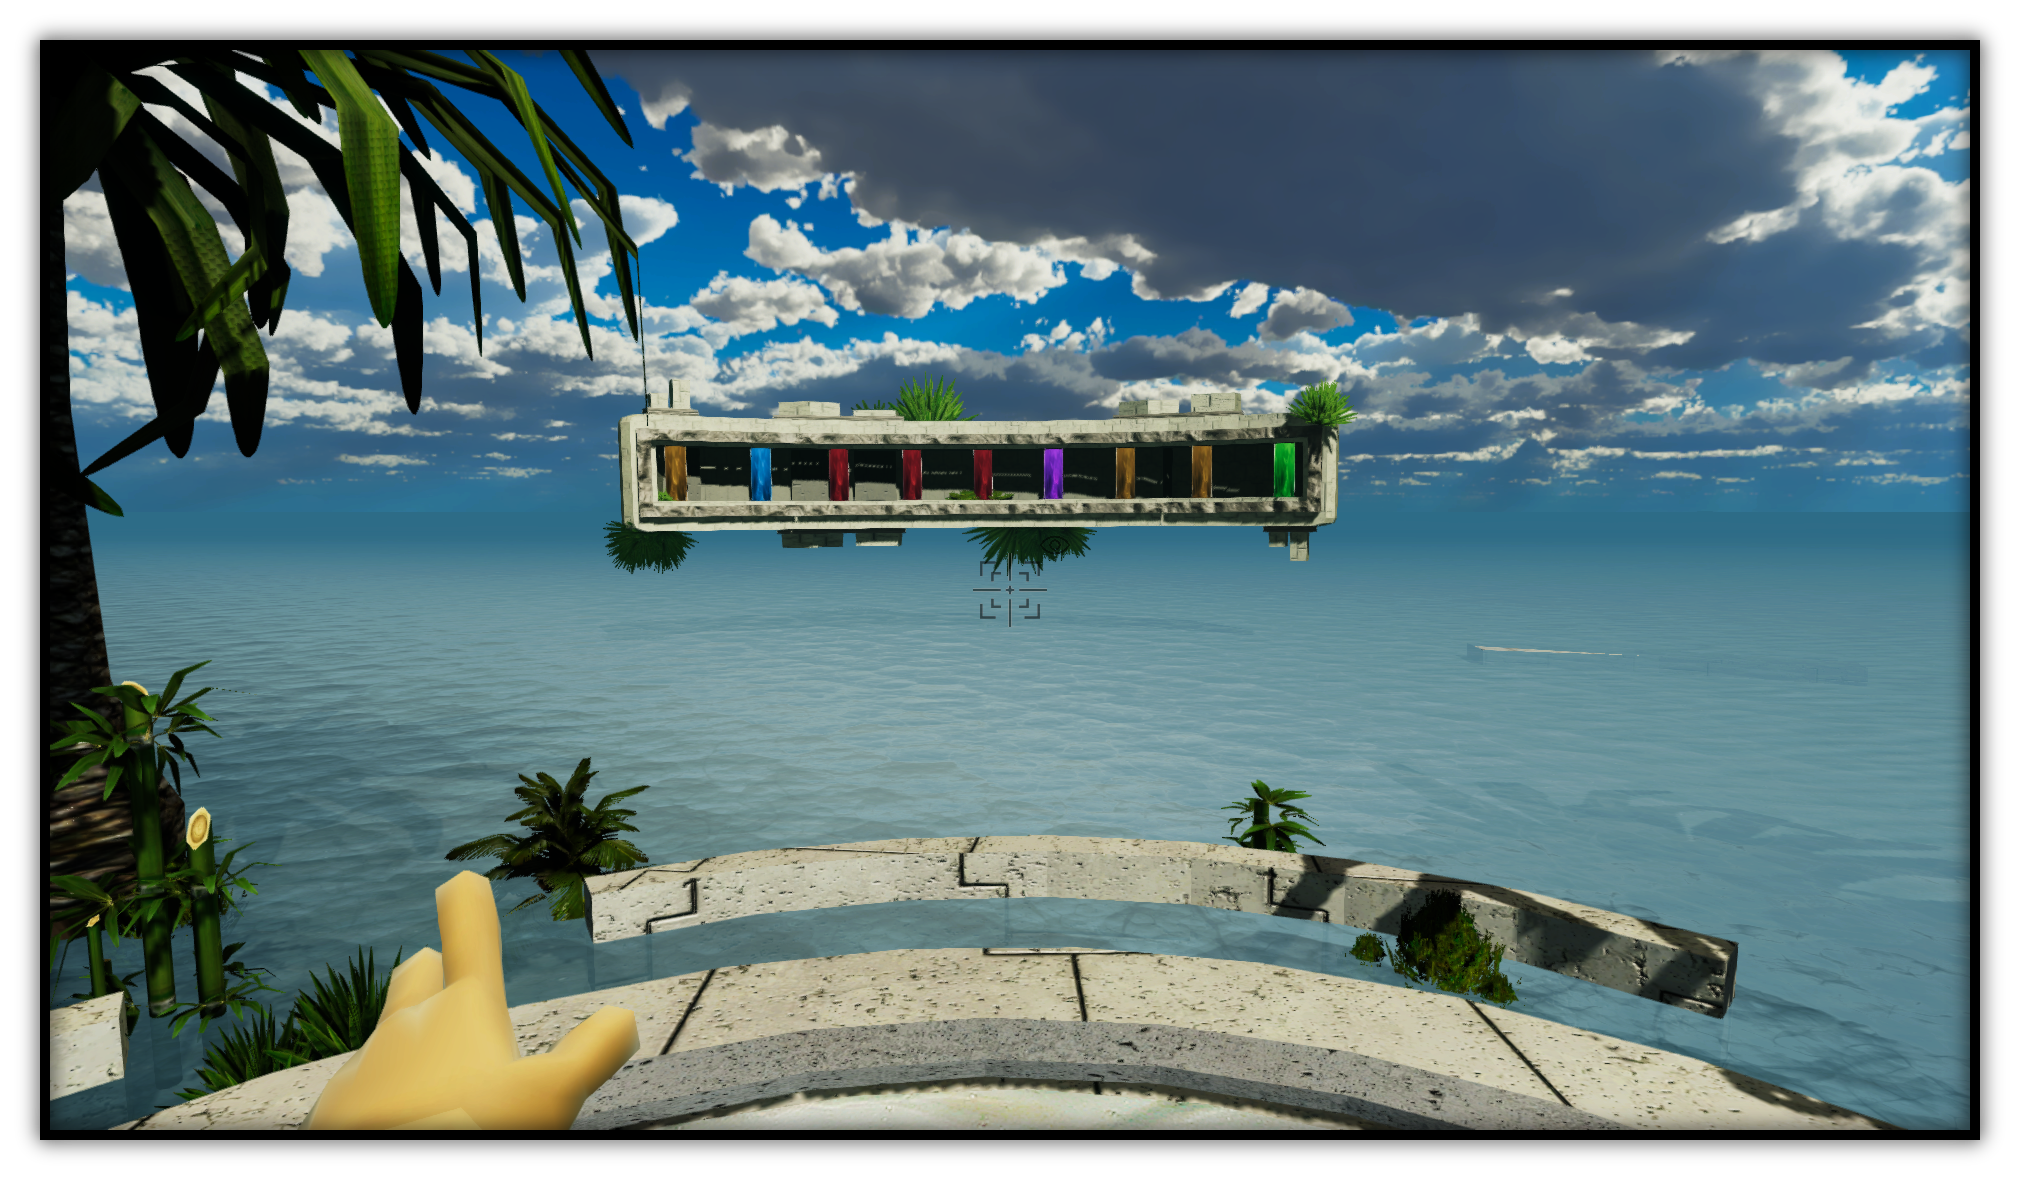
\includegraphics[width = \linewidth] {[ Figures ]/Sequence Mini-Game.png}
		\captionsetup{font = small, labelfont = small, width=.8\linewidth}
		\caption{Sequence: motor imagery based avatar control.}
		\label{fig:the_game_2}
	\end{subfigure}
	\captionsetup{font = small, labelfont = small, width=.8\linewidth}
	\caption{Screen shots of the game.}
	\label{fig:the_game}
\end{figure}

\pagebreak

The first, \reffigure{fig:the_game_1}, was a re-imagining of the arcade game Breakout \ccite{breakout}, in which the players aim is to break each block on the games board by bouncing a ball into them using a movable paddle, placed at the bottom of the play area. The intent with this part of the project was to allow the player to be able to effect the game world through an indirect influences, in this case, through the scaling of game difficulty. This was done by classifying the players state of relaxation and concentration, increasing and decreasing the ball's movement speed based what state the system determined the players focus to be.

\hfill

The second mini-game, \reffigure{fig:the_game_2}, had the player tasked with repeating a given sequence of colours back to the game, by activating crystals of the same colours in the correct order. This mini-game was used to explore the concepts of motor-imagery based avatar control. This was accomplished by requiring the player to activate a crystals by lifting one of the avatars arms up. To complete this, the player was required to think left-wards or right-wards. In doing so, their avatar would begin lifting the chosen hand forwards. 






\pagebreak
%System Inputs
\subsection{System Inputs}	

%Research into the different input methodologies demonstrated 


\begin{figure}[H]
	\centering
	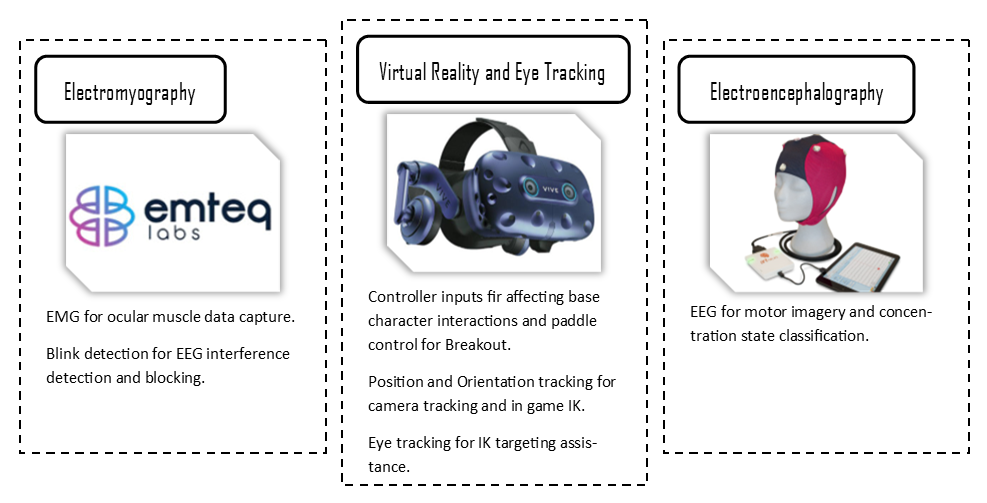
\includegraphics[width = 0.9 \linewidth] {[ Figures ]/System Diagram - System Inputs.png}
	\captionsetup{font = small, labelfont = small, width=.8\linewidth}
	\caption{System diagram: The input devices for the entire system.}
	\label{fig:system_diagram_:_inputs}
\end{figure}


\subsubsection{EEG}	

The recording of live EEG data is achieved through the sampling of voltage potentials across a subject's scalp, which is typically performed via the use of a high resolution sensor array. The signals collected from these sensors are then collated within an amplifier, such as the EEGO Sport, and accessed in the form of a stream of float channels, usually one channel per sensors. Finally to record this data the amplifier is then connected back to a host computer, in which the saving and recording of the data is completed. The usage of this technology within the project will be specifically for motor imagery, and the classification of relaxation and concentration states. Accessing this data live will be discussed in the networking part of this dissertation, however worth noting is that, due to the impractical nature of constant EEG tests, the large majority of this project was built around spoofing live EEG data using offline recordings downloaded from open access databases \ccite{albasri2019eeg} \ccite{goldberger2000physiobank}. The specific ways in which this will be achieved will also be covered later in this dissertation.


\subsubsection{EMG}	

EMG is the recording of the voltage given off from the activation of motor neurons within the body. By placing these sensors across the certain regions of the body, the activity of muscular movements can be recorded and understood. The use of this technology within this project was focused around the eye, where it was used to detect when the player would blink. The purpose of this was to be able to detect and cease the effects of any EEG data on the game during the times a player blinked, this was seen as a requirement to the large amount of interference the movement of facial muscle can cause upon EEG recordings. In parallel to that of the EEG, pre-record sessions of eye motion EMG data was also used in the stead of requiring access to live data each time the project need to be tested \ccite{bhpj-mz94-21}.


\pagebreak

\subsubsection{VR}	

Though this system was initially intended to be built for the HTC Vive Pro Eye, with Unity's XR Interaction Toolkit package, the specific headset used alongside the project is a bit less consequential. This is due to XR Interaction Toolkit's new input system, in which interactions are adapted to action bindings, rather then using string look-ups or the Input class for accessing the state of specific keys. Using this package, tracking data accessed from almost any headsets can be very easily bound as an action in the interaction asset. However, a headsets does require a project to be built for a specific platform, such as Android or Windows. With the intent of building this project for the HTC Vive however, the build platform can remain as Windows. In addition, this allowed for a mouse and keyboard solution to also be integrated into the project, to replace the inputs given via the headsets. This was important as it allowed for faster and less cumbersome testing of the solution. This replaced the headsets orientation tracking with a parametric based look function controlled via the mouses movement delta, as well as control over the paddle in breakout using the `A' and `D' keys, instead of inputs from the headsets controller.




\pagebreak
%Network Data Transfer
\subsection{Cross Network Data Transfer}
	
Unlike accessing data from both the VR headset and the Emteq Pro, where both maintain a direct physical connection to the games host device, accessing EEG data is more complicated. As stated previously, sampling EEG data is done through connecting the sensors to an amplifier and then the amplifier to a separate computer for recording, however to maintain an undisturbed and interference free sample collection this system must be separate from that of the system the game is running on. This creates a new problem, how to access the data generated on a separate machine across a local network, and more specifically how to access this data in as close to real-time as possible.


\begin{figure}[H]
	\centering
	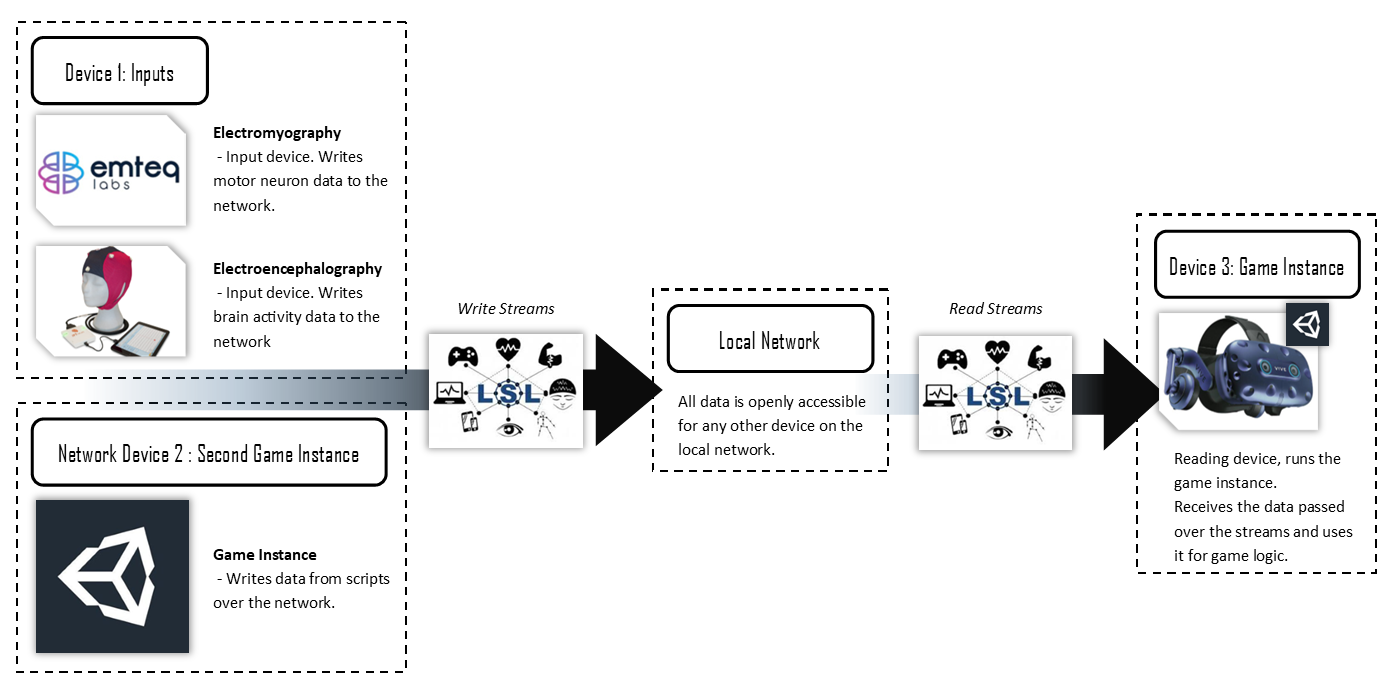
\includegraphics[width = 0.9 \linewidth] {[ Figures ]/System Diagram - Network Transfer.png}
	\captionsetup{font = small, labelfont = small, width=.8\linewidth}
	\caption{Data transfer across the local network using the LSL protocol.}
	\label{fig:networking_diagram}
\end{figure}


\subsubsection{LSL}	

The solution was the LSL (Lab Streaming Layer) protocol \ccite{labstreaminglayer}. LSL offers time-synchronous multi-type data transfer across local networks. Fortunately systems like the EEGO Sport come with software that supports this protocol by default, this has allowed for the distribution of all live data recorded from the head-wear to be accessed by any device on the network.

  
\subsubsection{Integration with Unity}	

However, though the broadcasting of EEG data via LSL, using software like EEGO, is inconsequential, accessing these streams within Unity requires a bit more work. To do this the 'liblsl-Csharp' package was used. This package allows for the integration of the LSL protocol into Unity through C\# scripting, requiring only the inclusion of the provided LSL.cs file, a C\# scripting file, and a specific .dll, library file, matching the games build platform. The library file used in the project is determined by the VR headset that a game is being built for, in the case that this projects aims to build on a device like the HTC Vive, the required library was LSL's Windows .dll. However for headsets like the Pico G2 4KS and the Oculus Quest, an Android based library will need to be built for the specific version of Android these headsets are running. 

\hfill

With LSL working within the engine, the objective for getting working scripts for both the writing and recording of LSL streams became a priority. To do this, two abstract classes inheriting from the Unity class MonoBehaviour were written, LSLInput<T> and LSLOutput<T>, where T was the channels data type provided through the child class. 

\hfill

The LSLInput class was designed to contain information on the type of stream Unity would try to listen for, this included two serialised fields for protected strings, of which were used to store the stream's name and description. On top of this an Enum variable would also be assigned, this would tell the classes inheriting from LSLInput whether to listen into streams with a matching name or description when searching the network.

\hfill

An example of one of LSLInputs child classes is the LSLInputStream\_FloatArray class. This class used a float as the template data type of it's parent, this set the data type of the samples received from all input channels to all be considered as the type float. The class was designed to continuously search for an LSL stream, using the search terms provided, and upon finding a match would begin pulling the data from it at the same rate as it would be being written. This allowed for the usage of input streams that did not match the frame rate of the game. On obtaining the sample, the float array is stored in a read only public list, accessible to any other scripts within the program that may require this data.

\hfill

Like the LSLInput class, the LSLOutput was written to store two serialised strings for both the name and type of data being passed. However, unlike the LSLInput class, the child classes of LSLOutput were not designed to search for streams on the network, instead they were used to create and then write to their own streams. 

\hfill  

An example of this is the LSLOutputStream\_PositionData class. Upon starting the game, this class is used to generate a new LSL stream containing three channels, each holding floating point numbers as their data type. These channels labelled `X', `Y' and `Z', were written to every fixed update with the position of the game object this script was attached to. By attaching this script to a game object and playing the game, the reading of this objects position could be read from anywhere across the local network. Either from a separate application, such as BrainVision's LSL Viewer, or from another instance of the game where the LSLInput script is used.


\begin{figure}[H]
	\centering
	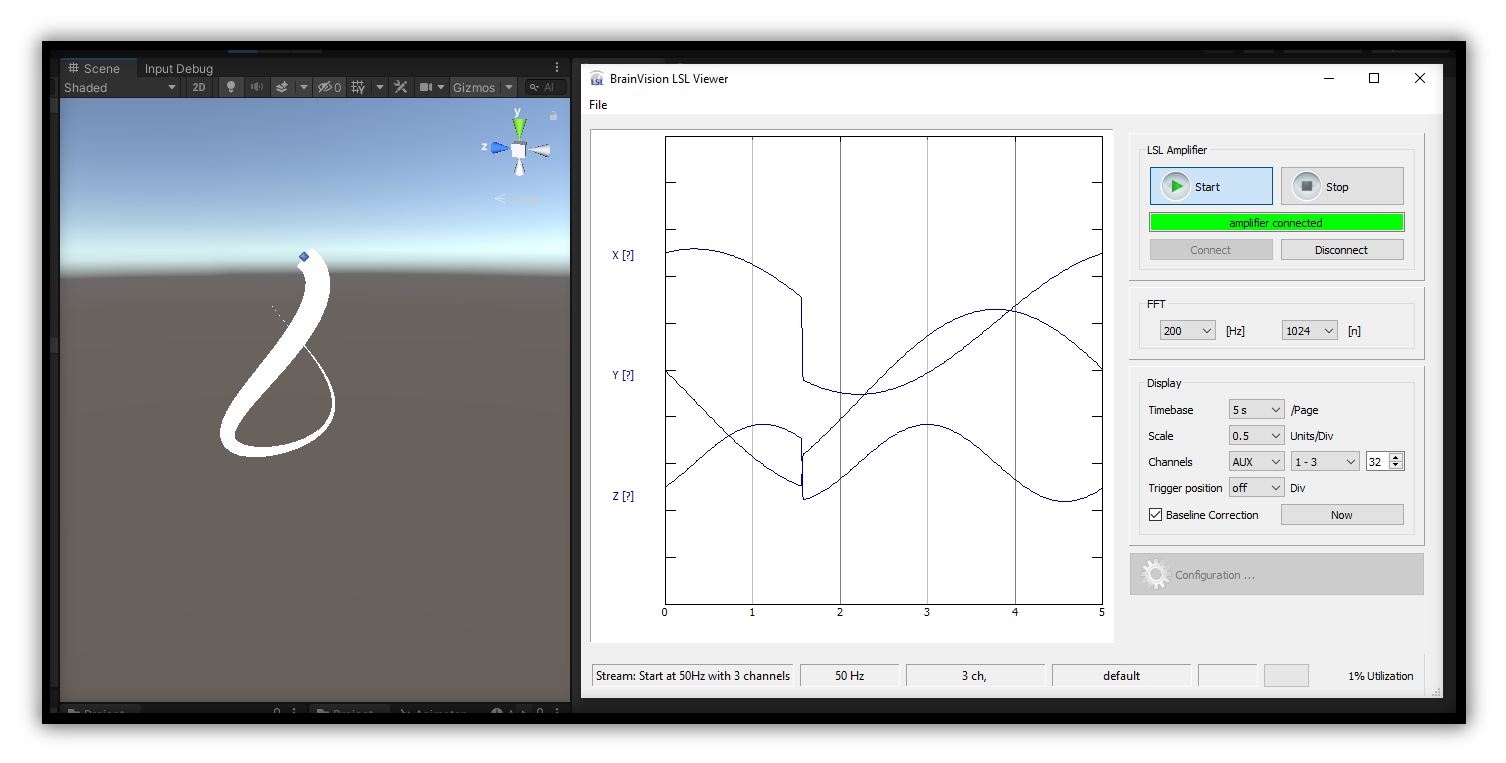
\includegraphics[width = 0.9 \linewidth] {[ Figures ]/Brain Vision LSL Viewer.png}
	\captionsetup{font = small, labelfont = small, width=.8\linewidth}
	\caption{Brain Vision LSL Viewer visualising the motions of a moving game object in Unity.}
	\label{fig:LSL_output_position}
\end{figure}

\pagebreak

Using this script, the potential for spoofing real time data through the re-writing of a pre-recorded session for both EEG or EMG over the network was possible. With this, the requirement of having a participant running through the game with the entire set up, EEG, EMG and VR headset became unnecessary. Instead, for creation of a prototype, spoofed online data could suffice.

\hfill

To do this, an child class of LSLOutput was written. This new child class contained a serialised field for a TextAsset, in which a CSV (Comma Separated Values) file filled with offline EEG or EMG data could be inserted. Each column in the CSV file was acted as a channel of the input data, while each row acted as an individual sample. The sample rate was also taken as a serialised field, this allowed for the data to be streamed over the network with varying frequencies, allowing for the close match for that of the original recording frequency. On game start, the script would convert the contents of the attached CSV text asset into a string, by manually separating the contents into a two dimensional list, matching the rows and columns of the file. After which an LSL output stream would be established, with the channel count equal to the width of the two dimensional array. Subsequently, each frame a new sample would be pushed from the list and streamed over the network. Resulting elsewhere in the same input streams from that or a real data capture device.   




\pagebreak
%Machine Learning
\subsection{Machine Learning}
	
Even with the data from EEG and EMG both accessible within Unity, taking a meaning from it is complicated, and requires a more involved solution. Taking these inputs at face value, with both the EEG and EMG, each time a sample is taken, a series of float values are returned in the form of an array. Where each index of the array is considered a separate channel. Manually testing these numbers within Unity was not a viable solution, the large quantity of channels and the apparent randomness appearing as the values from each made the contents of the sample somewhat meaningless. Instead, an analysis over the whole collection of channels was required, to accomplish this, the project opted for the use of pre-trained FFNNs within the game, this would allow for the discovery of patterns forming across the entire sample as a whole. 

\hfill

The FFNN architecture was chosen as the desired neural network due to the simplicity of creating one of these models, as well as their usefulness in simple classification models. With this architecture, three network models were developed, each was tasked with the classification of either the EEG or EMG streams. These networks consisted of: a motor-imagery classifier using EEG samples, specifically the network was trained to classify the likelihood between an imagined left, right and neutral state; a concentration based network, in which the EEG data was once again used, this time however to determine between the likelihood of a relaxation or concentration state; while lastly, the final network used samples from the EMG data to classify between the action of opening or closing a players eyes.


\begin{figure}[H]
	\centering
	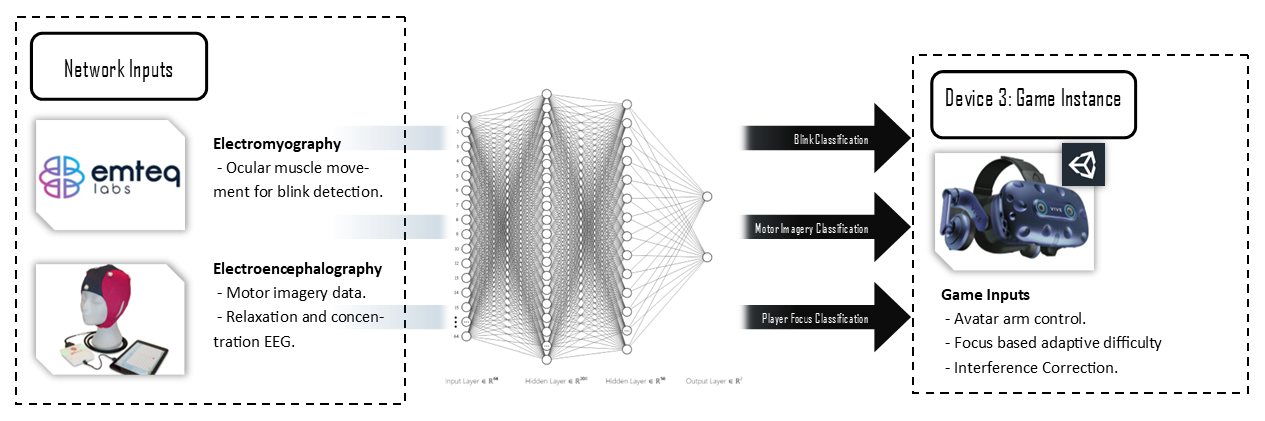
\includegraphics[width = 0.9 \linewidth] {[ Figures ]/System Diagram - Machine Learning.png}
	\captionsetup{font = small, labelfont = small, width=.8\linewidth}
	\caption{Artificial neural networks, there inputs and outputs.}
	\label{fig:system_diagram_:_machine_learning}
\end{figure}


\subsubsection{Keras}	 

To create these networks the Python library Keras \ccite{keras} was used. Keras is an interface library for Google Brains TensorFlow \cciteyear{tensorflow}, another python library used for the creation and training of neural networks. Using the offline motor-imagery, relaxation and focus, and eye movement data sets mentioned in Section 5.1, a model using the `Binary Cross-Entropy' algorithm was generated for each. These models were originally designed with a hidden layer 20\% the size of the input layer, as shown in \reffigure{fig:ffnn_:_original_motor_imagery}. However the results of this network after several hours of training didn't appear promising. The networks accuracy remained unaffected by any increase in epochs, continuing to remain at 50\%. A percentage that for a binary classification network with it's training data evenly split between it's expected two outputs, could have resulted from either a situation where: all outputs are the same no matter the input; or when the pattern the network has settled on outputs resulting values no better then random chance. 


\begin{figure}[H]
	\centering
	\begin{subfigure}[t]{0.45\linewidth}
		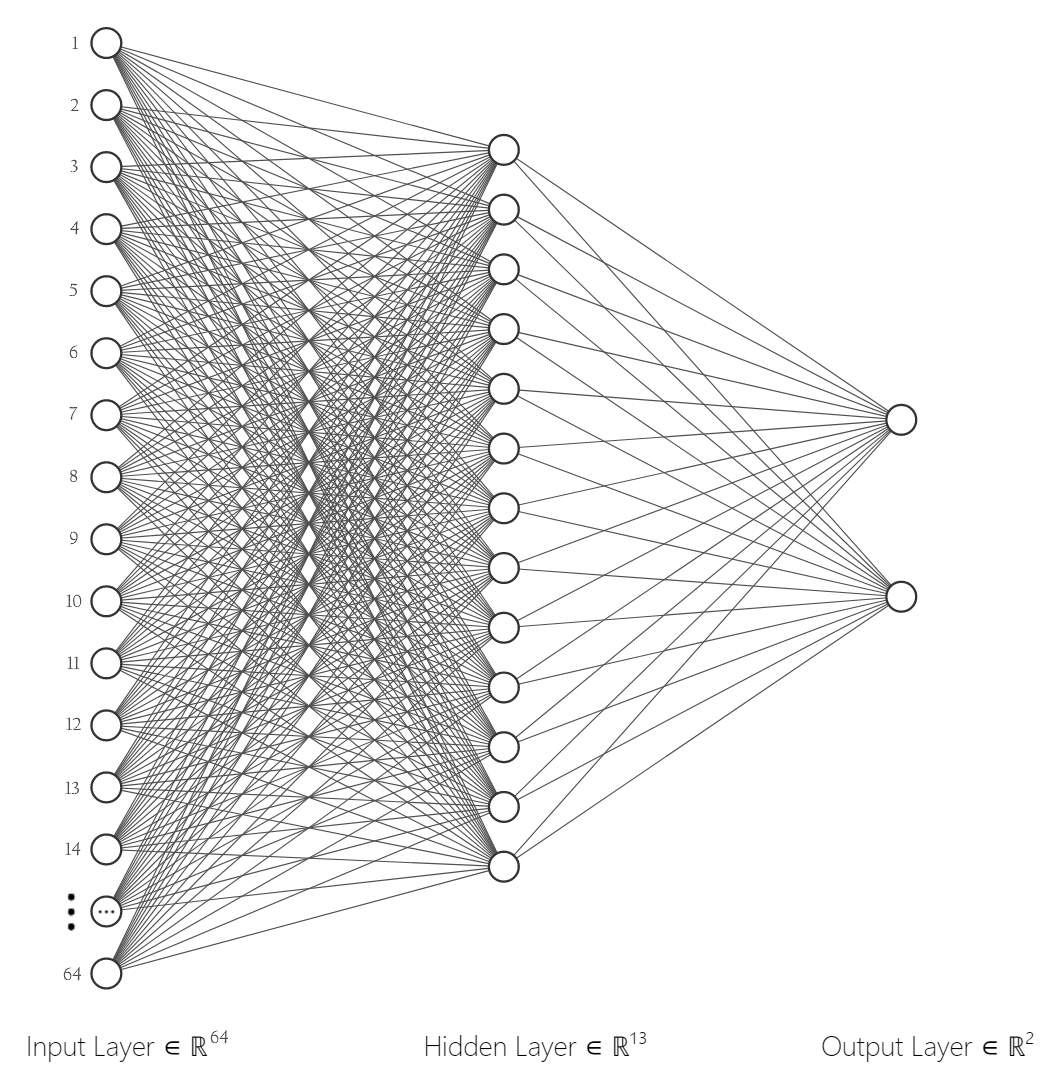
\includegraphics[width = \linewidth] {[ Figures ]/FFNN Original.png}
		\captionsetup{font = small, labelfont = small, width=.8\linewidth}
		\caption{Example of the original FFNN used in the project.}
		\label{fig:ffnn_:_original_motor_imagery}
	\end{subfigure}
	\begin{subfigure}[t]{0.45\linewidth}
		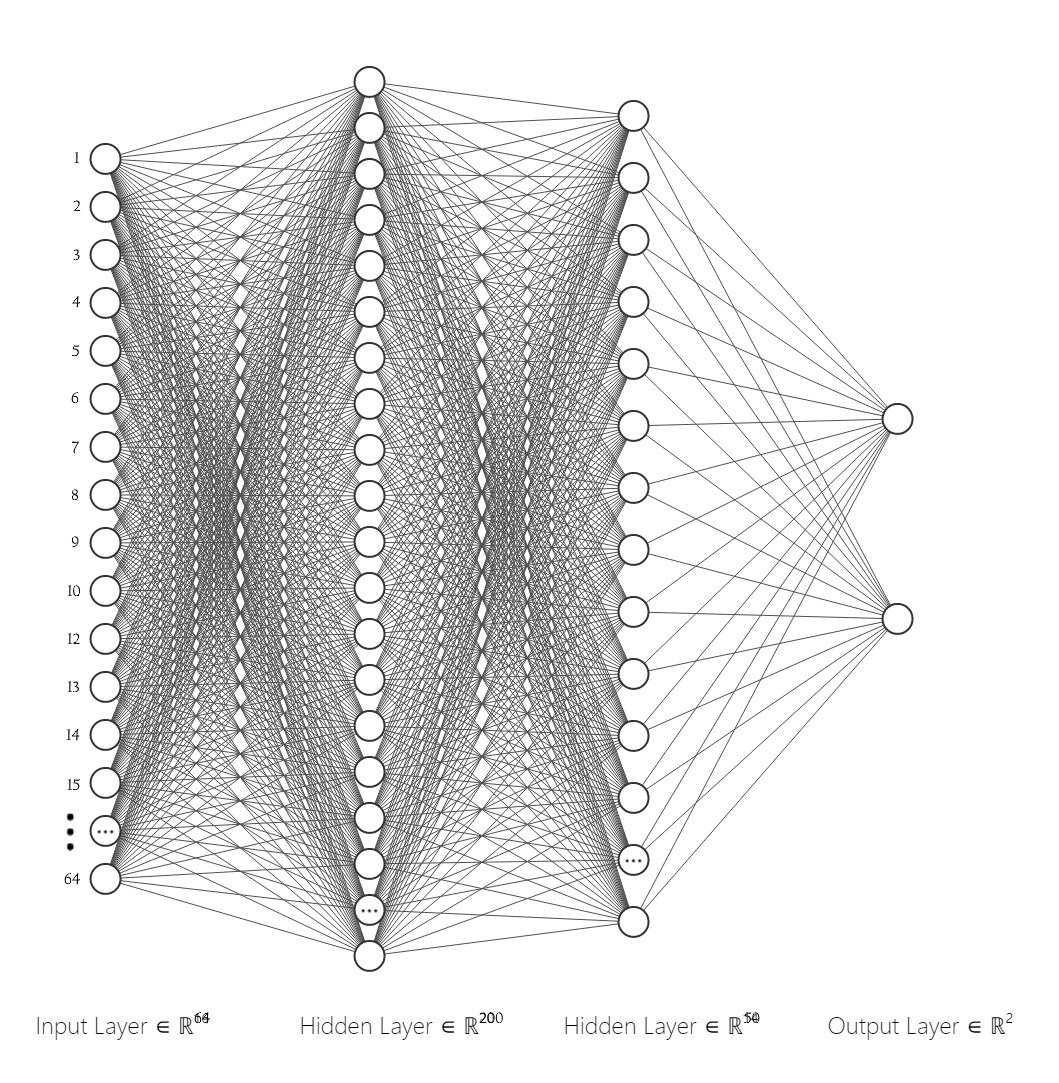
\includegraphics[width = \linewidth] {[ Figures ]/FFNN Second Attempt.png}
		\captionsetup{font = small, labelfont = small, width=.8\linewidth}
		\caption{Example of the updated FFNN using more hidden layers, where the size of each is also larger.}
		\label{fig:ffnn_:_200_node_layer_motor_imagery}
	\end{subfigure}
	\captionsetup{font = small, labelfont = small, width=.8\linewidth}
	\caption{Manually designed networks, figures generated using NN SVG \ccite{LeNail2019}.}
	\label{fig:ffnn_:_networks}
\end{figure}


Instead, the trialling of network architectures designed with more varied shapes and larger epoch counts began. Quickly, the base accuracy of these networks appeared to increase, the most favourable of which were the networks containing at least 2 or more hidden layers, and where the hidden layers first layer consisted of a node count exceeding 200.

\hfill

However, this still didn't solve the issue, even with the higher accuracy networks, some even sitting at around 90\% when compared with data the network has seen before, when compared against unseen (validation) data these accuracies greatly dropped. Becoming equal to no better then that of random chance. 


\subsubsection{Keras Tuner}

Due to the lack of validation accuracy given by the manually designed FFNN's, it appeared unlikely that with the continued testing of more manually designed networks a resulting validation accuracy would be close to being usable. On top of this, with the large amount of time required for giving each network a fair trial, it was clear that another solution was again needed. This emerged from the use of hyper-parameter optimisation, through the library Keras-Tuner \ccite{omalley2019kerastuner}. Keras-Tuner allows for the automatic search for high validation accuracy neural networks by parametrising the inputs used in the creation of a networks architecture. Then by iterating over these architectures using various search algorithms, the library is able to find the best ones. 

\hfill

There are 3 types of tuner algorithms supported by Keras-Tuner, `Random Search', `Hyperband' and `Basyesian Optimisation'. Testing was performed to determine which of these algorithms would result in the highest accuracy networks, in the fastest possible times. Over this testing period, the choice was made to utilise the basyesian optimisation tuner for the networks because this option showed the most success in consistently predicting networks with a high validation accuracy quickly.

\pagebreak

The final hyper parameters used in tuners are shown in \reftable{tab:ffnn_:_search_parameters}. Initially, with the EMG data, the generated networks showed exceptionally high prediction rates for calculating the likelihood of a blink action. However, for both the motor imagery and concentration models, the networks still continued to struggle with the unseen validation data. Resulting in the misclassification of the data. However, since these networks showed a high accuracy when comparing against any of the data they had been previously trained against, their use within the game when only using this data as an input meant the system could still be prototyped.


\begin{table}[H]
	\centering
	\begin{tabular}{ |c|c| }
		\hline
		
		Parameter 								& Value 							\\	\hline \hline
		
		Objective 								& `val\_accuracy' 					\\ 	\hline
		Layers 									& 1 to 6 							\\ 	\hline
		Nodes 									& 4 to 512, in steps of 4 			\\  \hline
		Hidden layer activation function 		& `relu', `sigmoid', `softmax' 		\\	\hline
		Output layer activation function 		& `relu', `sigmoid', `softmax' 		\\	\hline
		Learning rate 							& 0.01, 0.001, 0.0001 				\\	\hline
		Early stopping callback rate			& `val\_loss' 						\\  \hline
		Early stopping patience					& 3 								\\	
		
		\hline		
	\end{tabular}
	\captionsetup{width=.8\linewidth}
	\caption{Input parameters used for tuning network search generation.}
	\label{tab:ffnn_:_search_parameters}
\end{table}


\subsubsection{Baracuda}
	
With the networks generated, their implementation into the Unity game engine became the next step. Unity comes with two neural network packages built into it's package manager. The first of which is `Unity Machine Learning Agents', this package focuses on the implementation of machine learning in intelligent AI controllers for non-player characters. The second is `Barracuda', this package was chosen for implementation. Barracuda is a neural network interface library used for the implementation of pre-trained neural networks into C\# files. 

For the networks to be usable with Barracuda, each network had to be converted from TensorFlow's .h5 format into the .onnx format. This was handled within Python using the `keras2onnx' package. 

Once the networks were compatible with Barracuda, C\# scripts were written to accept the models and run them. Working with Barracuda in C\# requires the containment and set up of multiple classes within the package, the class Barracuda\_Model, was written to interface with Barracuda and store the necessary classes as private fields. Setting up the network required the creation of a Model class through loading in the .onnx file stored within assets, this was accessible through assigning the file to a public NNModel field within Barracuda\_Model and calling the static Load function on the ModelLoader. A worker, used to run the network, was also created through the static CreateWorker function within WorkerFactory.

\hfill

With a model loaded, to pass data into it and retrieve an output the creation of both input and output Tensor is required. A tensor in mathematics is described as an n-dimensional list of numbers, vectors or other tensors, or as defined by Oseledets \cciteyear{oseledets2011tensor} ``Tensors are natural multidimensional generalizations of matrices''. In the case of the models used with this project, both input and output tensors consist of a one dimensional tensor containing the float representation of a number, where the length of each tensor may vary. To create the input tensor, the classes constructor is used, taking as it's parameters the size of the desired network's input layer, alongside a float array containing the input data that will be ran through the network. It is then possible to generate the network output tensor by calling the Excute function on the model's worker using the input tensor as a parameter, then finally calling the Peek function on the object that is returned.

The output tensor contains information on the networks prediction, this information comes from the finalised values of each node in the networks output layer. To access this data easily alongside what output each network would predict to be most likely, the Prediction class was written. This class encapsulates the functionality of retrieving the data from the tensor and searching it for the networks predicted output, other classes using this can then access a network's results when processing their own logic.     

\hfill

Once the integration of neural networks were working within the engine, a showcasing script for motor imagery data classification named MotorImageryPlayerController was written. This script was placed as a component on top of one of Unity's primitive cubes. Alongside the script an LSLInputStream\_FloatArray component, set to listen for motor imagery streams, and a RigidBody component were added, both of which were accessable from within MotorImageryPlayerController via private fields. On the game start, the MotorImageryPlayerController Awake function would call the set up functions for it's Baracuda\_Model object, populating it with the neural network trained for motor imagery. Each game update, the script would then attempt to access a sample from the LSLInputStream\_FloatArray and using it, populate an input tensor and run the network. After accessing the networks prediction, the cube would then be moved via its RigidBody component left or right depending on the prediction output. This test was successful, the motor imagery data allowed for the control over the movement of a cube in 3D space.  


\begin{figure}[H]
	\centering
	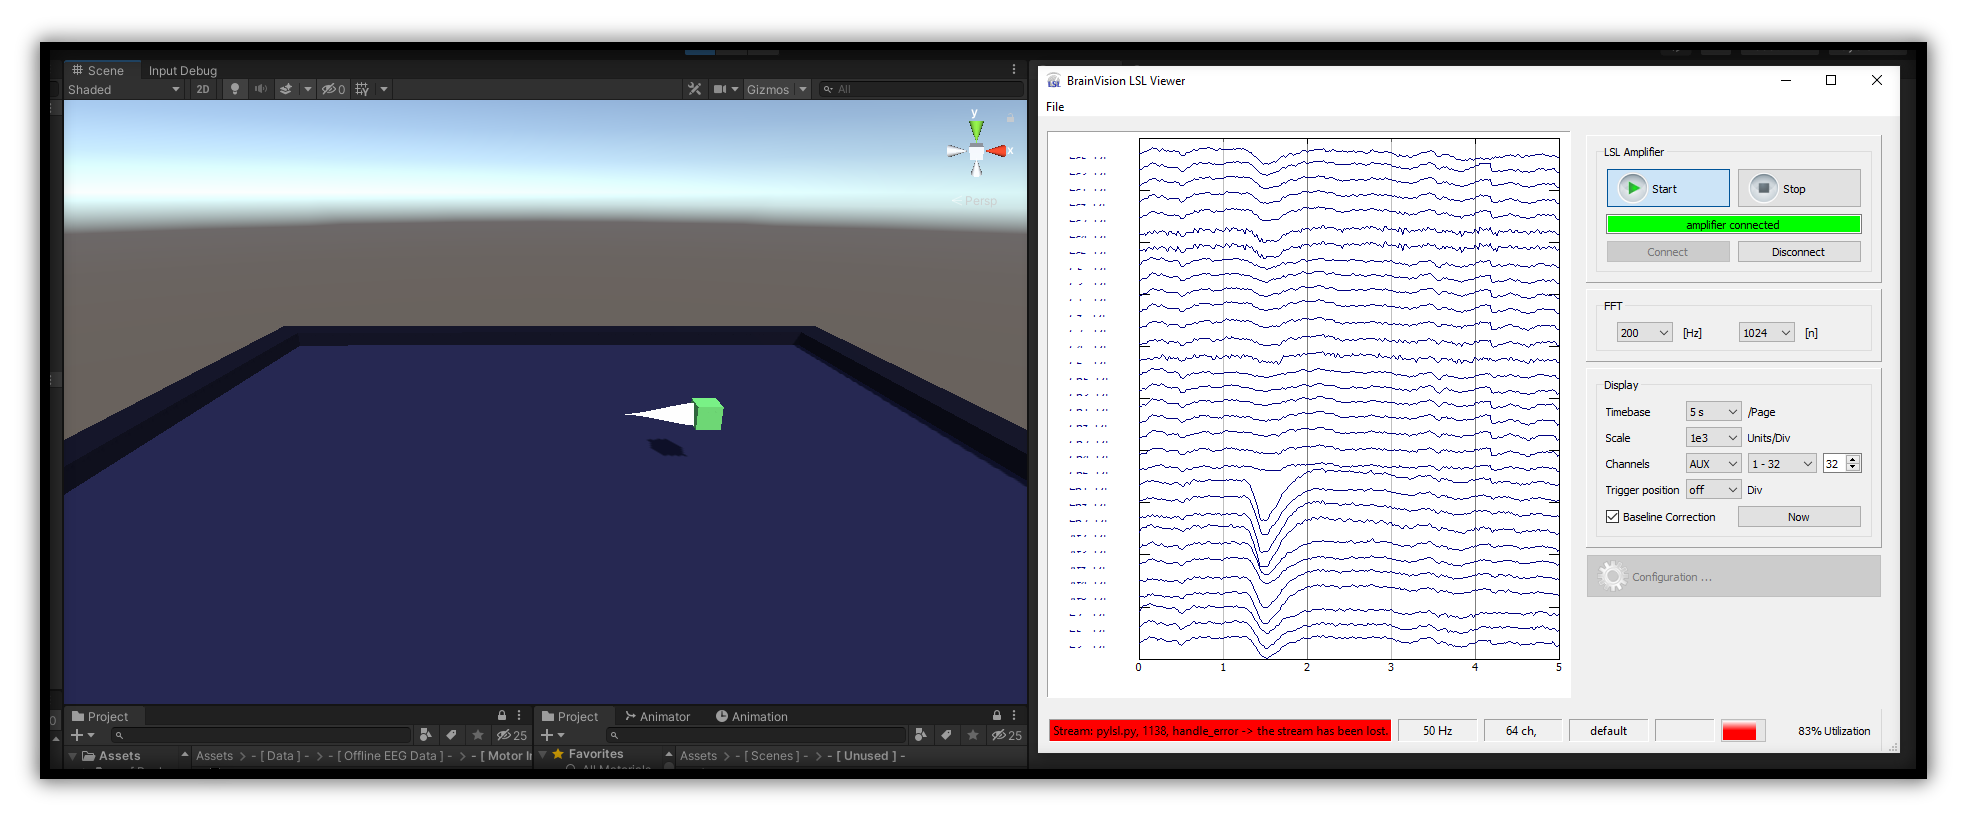
\includegraphics[width = 0.9 \linewidth] {[ Figures ]/Motor Imagery Test.png}
	\captionsetup{font = small, labelfont = small, width=.8\linewidth}
	\caption{Motor imagery controlled movement test for moving on a rigid body.}
	\label{fig:machine_learning_:_box_movement_showcase}
\end{figure}






\pagebreak
%The Games
\subsection{The Implementation of the Game}

Though this project was initially designed to work as a live demonstration using a VR headset with the streaming of real-time EEG and EMG data. The necessity for these devices to be present when testing the prototype was no longer required. Instead, the game that was created for the project ended up being built for Windows PC platform, where the keyboard and mouse were used as the games basic input system. Alongside this, EEG and EMG data were both supplied to the game via the re-streaming of pre-recorded data.  



\subsubsection{Game and Scene Set up}
	
The game was set up to have the player load into a small island in the middle of an ocean, this decision was made to avoid the implementation of having the player move around a levels environment, due to the possible complexity designing around this may cause. Alongside this, the lack of solid ground around the player visually indicated to them that they should not be expected to move the position of their body or avatar while playing. This also meant there was the option to port the game back to a VR headset, because a VR controlled look system would be unaffected by how the level and mini-games were designed.  
	
\hfill

On the island the player would be shown two stone tablets, both indicating one of the two mini-games. Upon interacting with one of these tablets, the game would load in a new scene additively using PhysX 3.4.0 \ccite{physx} multi-scene feature. This would allow for the quick loading of new game objects, without an interruption occurring on any of the already loaded game objects hosted by the main scene, such as the player and LSL listeners. The second motive for using multi-scene loading in this way is due to the easy clean up of game objects upon the completion of one of the two mini-games through just detaching the additional scene. However, this required the code for both the player and how they interacted with the mini-games to be completely separated, as to avoid any crashes or the need for large validation checks within the code. As such, all intractable game objects were set up with the component that controlled their behaviour inheriting from the base class Interactable\_Interface, each of these child classes would then be required to create an implementation of Interactable\_Interfaces abstract function Activate. This allowed the player controller to only call the Activate function upon trying to interact with anything, without needing any references to game objects or their components.  

	
	
\subsubsection{Player Controller}

User interactions within the game were managed through the control script Player, this class was placed as a component on top of the game object of the player avatar. The class functioned as: a way of taking in user inputs, for those defined within the XR Interaction Toolkit as well as the EEG and EMG data streams received over LSL; calculating and updating the inverse kinematic (IK) systems tied to the players arms and transform; and lastly, managing the Player's state machine, used to determine how the Player component would use inputs to interact with the game at a given point in time.

\pagebreak

IK used on the Avatar was driven by the Animation Rigging package, this package allowed the control over the avatar's arms using target and hint nodes, both of which were driven through scripting within the Player class. The weightings of each constraint were updated every frame through Player's Update function, however the weight itself was calculated within the player's active state. The player state machine was set up to transition between 3 states, each defined by a child class of ControlState\_Interface:

\begin{itemize}
  \item ControlState\_Basic.
  \item ControlState\_CrystalSequence.
  \item ControlState\_Breakout.
\end{itemize}

The flow of the player state machine was determined by a write only variable that through using a public setter would call the state's transition functions, an exit function for the old state and the entry function of the new state. The state of the player control would change depending on what part of the game the player is currently in. 

\hfill

On starting the game, returning to the main menu or entering the results screen after a mini-game, the player would be transitioned to the basic control state. In this state, the player would use the left and right mouse buttons to move the arms of the player avatar. On lifting an arm fully, a raycast would be projected from the players camera forward. If an object with a component inheriting from Interactable\_Interface was hit, the activate function of the component would be called. 

\hfill

The transition to the crystal sequence state occurs immediately after selecting the tablet to play the memory sequence mini-game, in this state the player drops the control given to them via the mouse buttons. Instead, the player would control the their avatars arms by using the EEG data passed via LSL, this would then be used as the inputs for the motor imagery based neural network. After which the network is used to determine if the player should move their left or right arms, more on this will be covered in the section covering the memory sequence mini-game.

\hfill

The final state, breakout, is entered upon selecting the breakout mini-game in main menu. This state has the player lose all control over their avatar. However, interaction is still calculated, this instead comes through the sampling of EEG data for determining focus state. This will also be covered in more detail in the breakout mini-game section.

\begin{equ}[H]
	\large
	\centering
	\begin{align}
		d_x & = Sin(o_x) *  Cos(o_y) 	\nonumber 	\\
		d_y & = Sin(o_y) 				\nonumber	\\
		d_z & = Cos(o_x) *  Cos(o_y)
		\label{equation:camera_parametric}
	\end{align}
	\captionsetup{font = small, labelfont = small, labelformat = empty, width = .8\linewidth}
	\caption{Calculation for player look vector: where \(d\) is the resulting three-dimensional vector; and \(o\) is a two-dimensional representation of the total mouse movement since the games start.}
\end{equ}

\pagebreak

On top of the state specific behaviour the player controller is also used to manage two other things. The first is the camera's rotation controls. Though this is unnecessary for a VR based implementation, for the prototype build, a parametric equation was used to create the look vector needed for the generation of the camera's rotation quaternion. This equation, as shown by \refequation{equation:camera_parametric}, was updated upon mouse movement by using the XR Interaction Toolkit's action event subscriptions. The second behaviour run inside the Player component is blink detection neural network, this was ran every frame before any of the state specific behaviour is called. This allowed for the ability to ignore any data and subsequent changes in actions within the EEG based neural networks, as to block any avoidable interference within the EEG coming from the muscular movements within the face.


\subsubsection{Mini-Game: Memory Sequence}

The memory mini-game was designed to entice the player into reaching out and using their avatars limbs. This was done by locking typical input modalities, like the mouse buttons and keyboard, and requiring the player to use motor imagery to move the arms of their virtual body. This game type was chosen due to its avoidance for accurate and fast decisions, allowing the player to comfortably learn how to move their body within the virtual space.

\hfill

On loading into the game, a randomised sequence of specific colour types is generated and displayed to the player as a series of coloured crystals. This is done through this mini-game's controller script. Crystals matching each of the possible input colours where also spawned into the game, in a ring surrounding the player. Each of the crystal game objects possessed a component inheriting from Interactable\_Interface name Crystal, this component also contained a serialized field for an enum representing the crystal's colour, this was assigned within the unity inspector. On being targeted by a player interaction, through the raising of the players hands while looked at, the crystal will be considered activated and the colour will be sent to the mini-game controller script as an inputted value. On correctly matching a colour, the sequence will accept the colour and increase the sequence index, awaiting the next in the sequence. On matching all colours in the entire sequence in order correctly the mini-game will end and the player may exit back to the main menu. However, inputting an incorrect colour will restart the players progress, having them start again from the beginning.

\hfill

As mentioned before, movement of the avatar arms is tied to the player control state ControlState\_CrystalSequence. Each game update, this state retrieves an updated list of the current EEG samples collected by the LSLInputStream\_FloatArray component attached to the player. Iterating over this list, each sample is taken and then used within two separate motor imagery classification models, one for left-ward thinking, and one for the right-ward. This would allow for the potential of simultaneous arm usage. These outputs are then used to control whether they should lift their arms or leave them slack. 

\pagebreak

This implementation alone would not work however, the slight inaccuracies with even a well trained network would cause a constant misactivations of the crystals. Instead, the movement of each arm was tied to an activation value, ranging from zero to one. In the case that the networks would consider a direction chosen, instead of moving the arm up instantly this movement would be tied to a growth rate. Each frame of input, an arms activation would either increase by the growth rate, or decrease by half of the growth rate as shown in \refequation{equation:arm_activation}. 


\begin{equ}[H]
	\large
	\centering
	\begin{align}
		a & = max(0,min(a - (g / 2),1)) 	\nonumber 	\\
		a & = max(0,min(a + g,1)) 
		\label{equation:arm_activation}
	\end{align}
	\captionsetup{font = small, labelfont = small, labelformat = empty, width = .8\linewidth}
	\caption{Arm control growth rate: where \(a\) is the independent activation value of both the left and the right arms; while \(g\) is the growth rate of the function, equal to 0.05.}
\end{equ}


To solve the issue of any misactivations when lifting the players arms, the player controller was set up to only consider an arm activate upon its activation value rising greater then 80\%. Upon triggering an activation, the arm would then be unable to call a second activation until it's activation value falls back down to 30\% where it's state would be reset. This allowed the complete removal of any accidental activation when classifying the inputs with an inaccurate neural network.



\subsubsection{Mini-Game: Breakout}

For the second mini-game, the arcade game Breakout was used. This was due to the simplicity of the game's rules and the familiarity many have with the game. The mini-game was used as a means for integrating the multi-modal adaptive difficulty system into the game, the objective was to have the player indirectly control an aspect of the game by adapting to their state of mind. To avoid complications, other interactions within the game, like moving the paddle, were controlled via keyboard inputs `A' and `D'. These were set up through the XR Interaction Toolkits action bindings, allowing for the ease of rebinding in the future for VR headsets.

\begin{equ}[H]
	\Large
	\centering
	\begin{align}
		s = s_\mathrm{min} + (s_\mathrm{max} - s_\mathrm{min}) * f
		\label{equation:ball_movement_speed}
	\end{align}
	\captionsetup{font = small, labelfont = small, labelformat = empty, width = .8\linewidth}
	\caption{Ball movement speed equation: where \(s\) is the speed of the ball; and \(f\) is defined as players the focus activation}
\end{equ}

\pagebreak

Difficulty within the mini-game was defined by the movement speed of the ball. The speed of the ball was calculated as the linear interpolation between the ball's maximum and minimum speeds. as shown in \refequation{equation:ball_movement_speed}, where the variable of focus activation was used to determine the final output between these speeds. The focus activation is defined within the Player class, its value is recalculated each frame within the ControlState\_Breakout state. This calculation is done through the processing of EEG data received over LSL. Much like the method for classifying the motor-imagery data, an input tensor was created using these samples and fed into the model trained for concentration prediction. However, unlike before where the output index was used to predict a specific state, instead the weight of the final output was used directly to determine how focused the network believed the player to be. This was then set as the player's focus activation. Since this output was stored as a real number rather then an integer, it allowed for a much more fluid scaling of difficulty. 

\hfill

A visual demonstration for players focus activation was also provided when the breakout mini-game. This was created using world space canvas and scaling up an image using the same linear interpolation code as the ball's speed, though this time with different minimum and maximum values. This is demonstrated in the \reffigure{fig:focus_bar} below.


\begin{figure}[H]
	\centering
	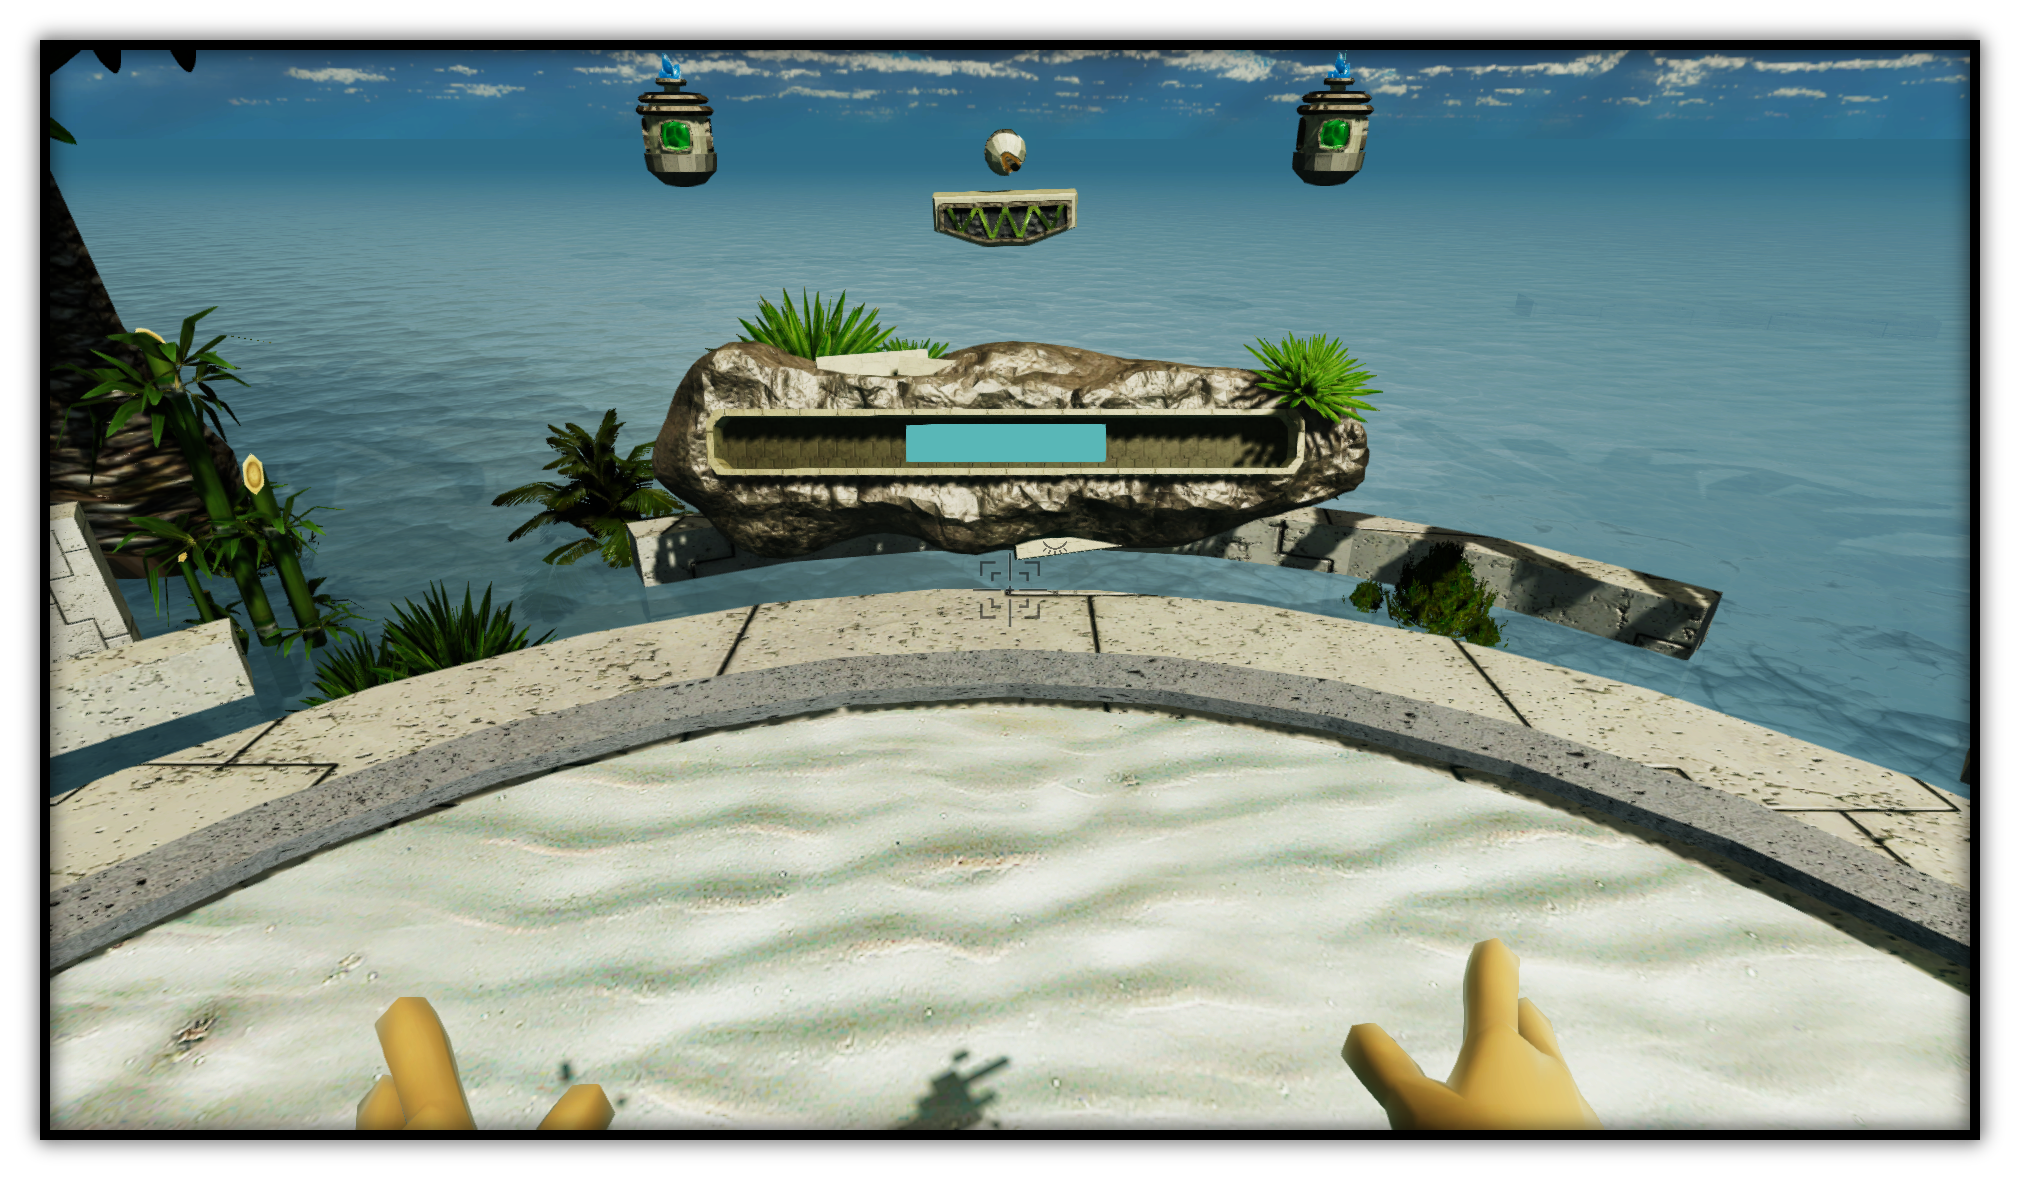
\includegraphics[width = 0.9 \linewidth] {[ Figures ]/Concentration UI.png}
	\captionsetup{font = small, labelfont = small, width=.8\linewidth}
	\caption{Concentration and relaxation controlled UI element.}
	\label{fig:focus_bar}
\end{figure}







\pagebreak
\section{Conclusion and Future Work}
\subsection{Conclusion}

Though the project ended up succeeding with the completion of a multi-modal system integrating EEG, EMG and a windows system, with the potential for VR testing. There wasn't however the option to test any of it using real live recordings and participants. On top of this, the neural networks used for both the EEG related systems only resulted in usable outputs when given data they had already been trained on. The most likely case is that the neural networks became over fitted for the input data and could not find a valid pattern within the larger picture, this may have been due to the limited sample size given to train on or that a more complex version of machine learning solution is required for a viable version of this system.

\hfill

Additionally, the two focuses of this project, being avatar control and adaptable difficulty, may have been better tested using a different implementation or game. The changing ball speed in Breakout alongside the visual display of the player's focus activation meant that in a real use scenario, players could learn to abuse the system by deliberately attempting to change there mental state to take control over the ball's speed. If a player could learn how to do this, it would go against the project objective of having the game automatically adapt to the players unconscious state of mind, with the purposes of increasing enjoyment and engagement. Secondly, the sequence mini-game also shared a similar issue. The mini-game was designed to allow for players to become comfortable in using either of their arms by giving them free choice in reaching out with whatever arm felt natural. This would ideally be used in the same way that a person would use the right arm or left arm to pick an object up in the real world depending on how the object is positioned relative to them. Instead, since the player is required to always look at the crystal they wish to interact with, it stands to reason that in the case of players, in which the system cannot accurately predict all of their inputs, they may learn instead to rely on one arm. Assuming that the networks outputs are of an on and off state, rather then the states left, right and neutral. 


\subsection{Future Work}			% - 300 Words

Continued development of this project would aim to solve many of the issues presented in the conclusion. The first would be the research and development of more complex EEG and EMG neural networks. The aim would be to both attain a much higher validation accuracy from the networks for their current purposes, while also investigating into further methods combining both these and other input methods, possibly even combining both technologies into a combined neural network. This however would require the project to have its own collection of new training data, since both the EEG and EMG could be would need to be comparable to the same stimulus or action.

\hfill

Incrementing on the project objectives tied to each mini-game, the improvement of adaptive difficulty would involve a better exploration and implementation of a less noticeable state change within the game. This would require the collection of either: a lot more data, possibly over the course of many frames; a greater number of more complex networks, each used to calculate a variety of potential variables tied to a players enjoyment; or even feeding this data into an evaluation profile of the player and by determining the players performance as shown by Yun and colleagues \cciteyear{yun2010pads} altar the game to best fit them. 

\pagebreak

As for the avatar control portion of this project, it would be of interest to have a greater look into the potential movement fidelity that a motor imagery based neural network may bring, while finding ways of making these networks more accurate. In the case of the mini-game itself, there are a multitude of possible improvements. The first involves the use of eye tracking and IK, with the intent of allowing the player to reach for objects not directly in front of them. Secondly, a look into the possibility of more accurate spacial imagination, this could allow for an IK system to move a players limbs to specific points in the space relative to their avatar rather then just forwards along specific vectors. Finally, changing certain objects to only be intractable with a specific hand of the players avatar, this would force players to become more adapt at using such a system rather then just relying on one arm.







\pagebreak
\printbibliography[notkeyword = software, title = References]

\pagebreak
\printbibliography[keyword = game, keyword = software, title = Games]
\printbibliography[notkeyword = game, keyword = software, title = Software]

\end{document}
